\documentclass{article}
\usepackage{graphicx} % Required for inserting images
\usepackage{caption}
\usepackage{subcaption}
\usepackage[a4paper,margin=2.5cm]{geometry}

\title{WBA_Aufgabe2}
\author{michael-kolle, thore-schwier}
\date{May 2026}

\begin{document}



\section{User Stories}

\begin{table}[h!]
\centering
\begin{tabular}{|c|p{2.5cm}|p{2cm}|p{4cm}|p{4cm}|}
 \hline
 Story & Titel & Wer & Möchte Was & Warum \\ [0.5ex]
 \hline\hline
 1 & Projekte erstellen & Projektleiter & Ein leeres Projekt erstellen & Um Aufgaben für Teammitglieder zu bündeln \\ 
 \hline
 2 & Projekte löschen & Projektleiter & Bestehende Projekte löschen & Um nicht mehr benötigte Projekte zu entfernen \\ 
 \hline
 3 & Projekte bearbeiten & Projektleiter & Bestehende Projekte bearbeiten & Um langfristig felxibel zu bleiben \\ 
 \hline
 4 & Übersicht Gesamtzeit &Projektleiter & Die Gesamtarbeitszeit meiner Projekte sehen & Damit ich die Zeitplanung verbessern kann \\
 \hline
 5 & Sortierung der Aufgaben & Projektleiter, Teammitglied & Die Aufgaben nach verbleibender Arbeitszeit sortieren & Die Abschätzung für den Aufwand zu vereinfachen \\
 \hline
 6 & Zeitabschluss & Projektleiter & Am Ende einer erledigten Aufgabe die tatsächlich benötige Zeit einsehen können & Falls nötig den Zeitplan anpassen und für zukünftige Projekte zu lernen \\
 \hline
 7 & Abhängigkeiten zwischen Aufgaben auflösen & Teammitglied & Die Aufgaben vor und nach einer Aufgaben sehen, wenn diese abhängig sind & Damit eine Aufgabe nicht zum bottleneck wird \\
 \hline
 8 & Projektübersicht & Projektleiter & Eine Übersicht über alle Projekte haben & Um schnell zwischen Projekten wechseln zu können \\
 \hline
 9 & Auswahl der Arbeitsschritte & Projektleiter & Bei der Planung eines Projekts aus verschiedenen Arbeitsschritten wählen & Um die Planung zu erleichtern \\ [1ex]
 \hline
 \end{tabular}
\end{table}

\section{Mockups}
\begin{figure}
\centering
\begin{subfigure}{\textwidth}
  \centering
  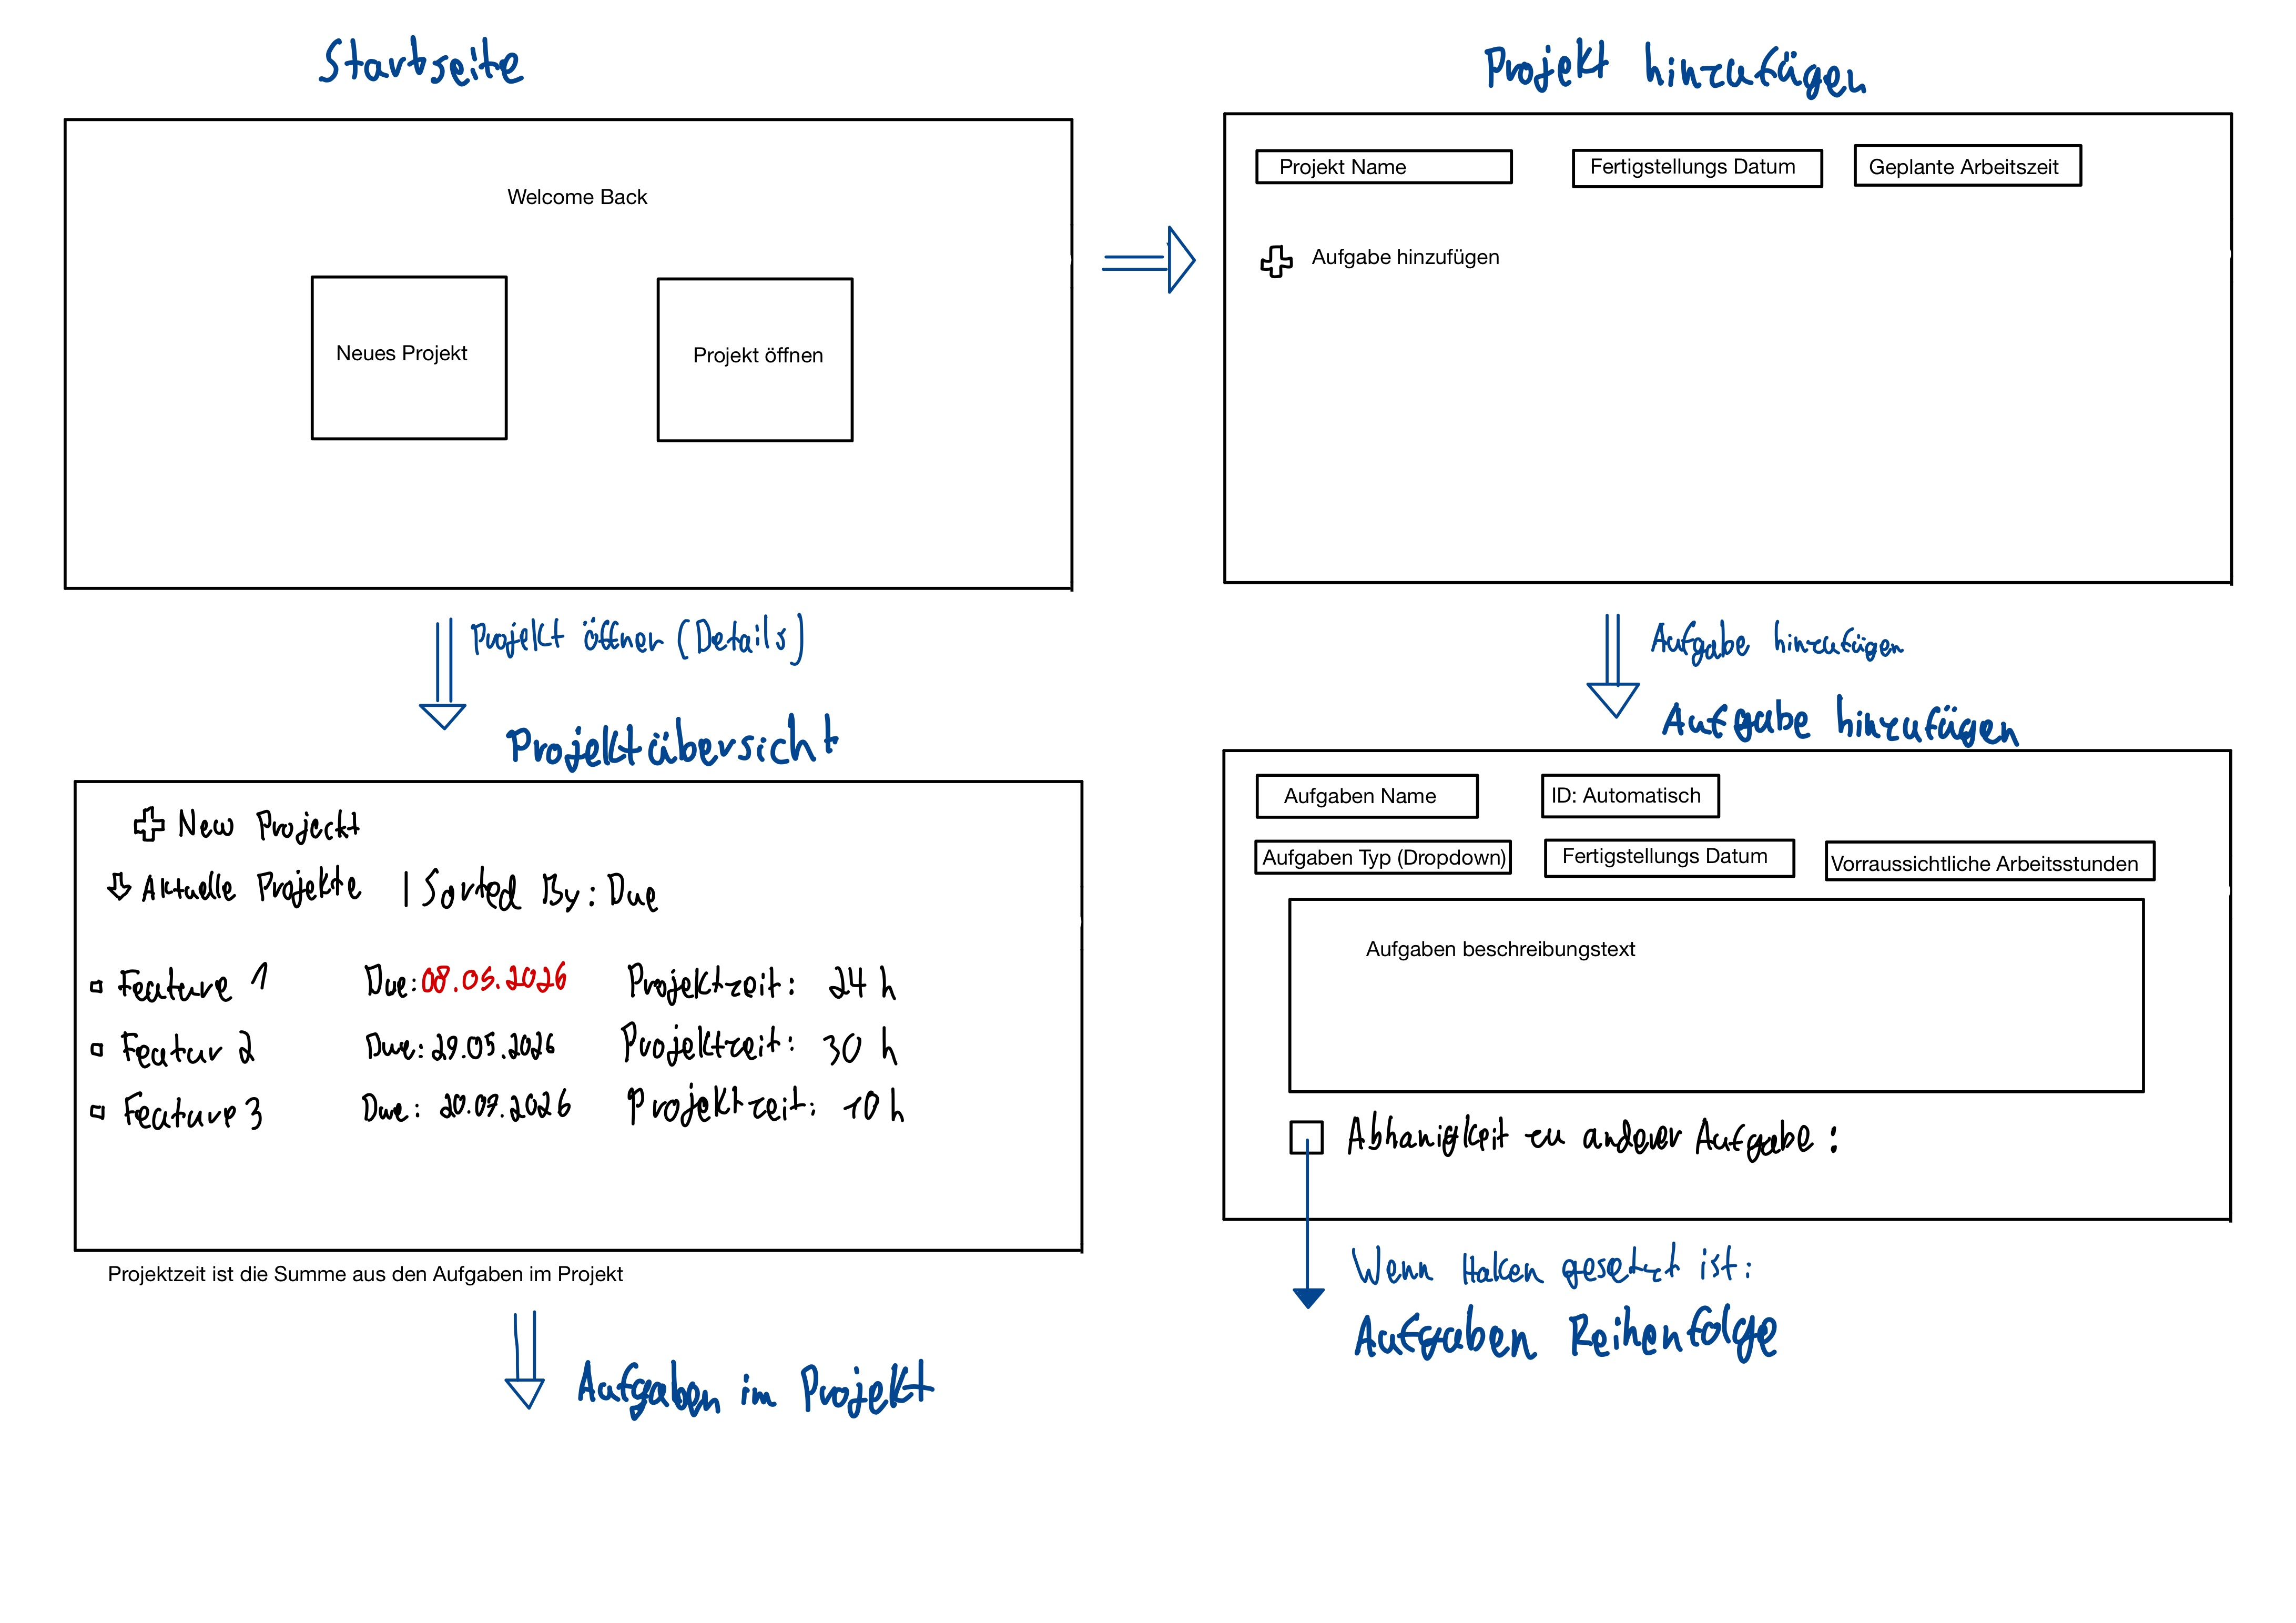
\includegraphics[width=\linewidth]{WBA_2_mockup-1.jpg}
  \label{fig:sub1}
\end{subfigure}
\begin{subfigure}{\textwidth}
  \centering
  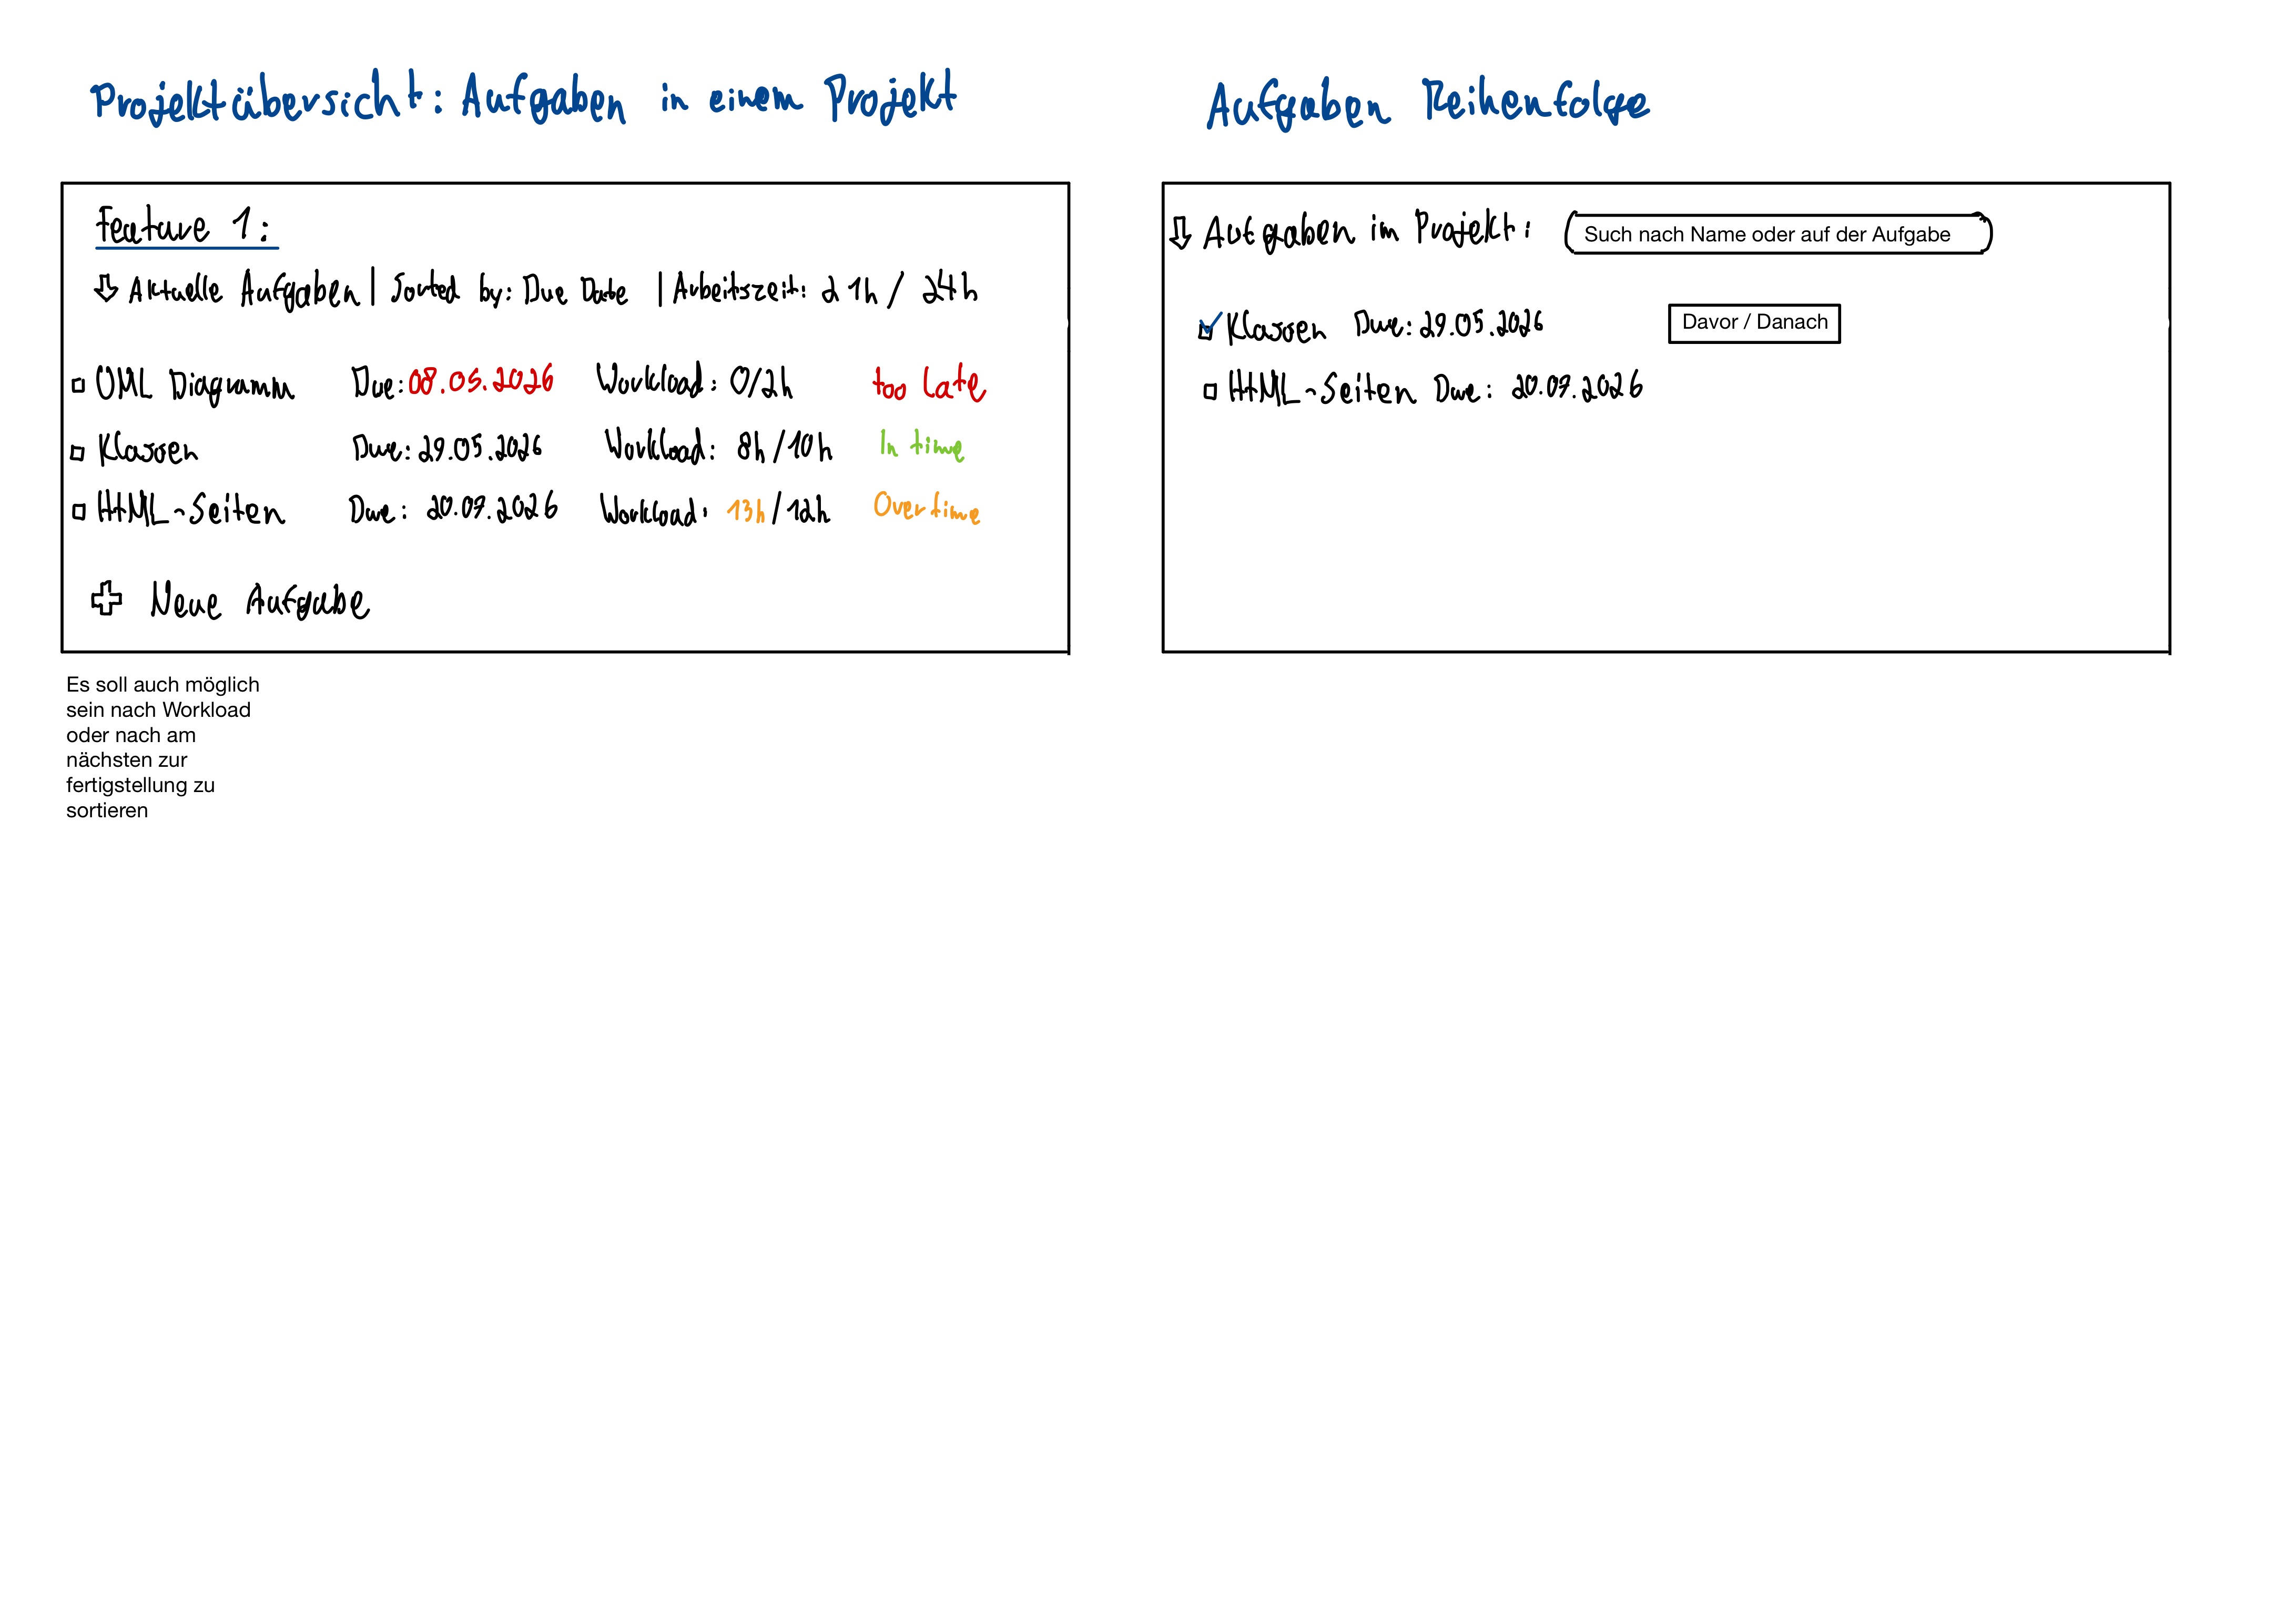
\includegraphics[width=\linewidth]{WBA_2_mockup-2.jpg}
  \label{fig:sub2}
\end{subfigure}
\caption{UI Mockup}
\label{fig:test}
\end{figure}

\section{Aufwandsabschätzung}

\subsection{Aufagbe a}
Das Projekt wird in kleinere Aufgaben geteilt.
Die Aufgaben werden nach Schwierigkeit, Aufwand, Art der Aufgabe (Design, Programmieren) gewichtet und eine geschätzte Zahl an Arbeitsstunden festgelegt.

Die Gesamtzeit ist die summierte Zeit aller Aufgaben, mit einem addierten Puffer.

\subsection{Aufgabe b}
Als Zahlen nehmen wir: 
Anzahl der Seiten für die User Story
Anzahl der Funktionen
Geschätzte Zeit pro Funktion
Zeit für das Design
Puffer Zeit für Fehlerbehebung

\subsection{Aufgabe c}
Generelles Setup: 5 Stunden
Startseite: 4 Stunden
Projektübersicht: 5 Stunden
Projektdetailseite: 3 Stunden
Seite für ein neues Projekt: 4 Stunden
Filter und Sortierung: 2 Stunden


\end{document}